\documentclass[border=10pt]{standalone}
\usepackage{tikz}
\usetikzlibrary{trees,calc,shadings,shapes.gates.logic.US,positioning,arrows}


\begin{document}

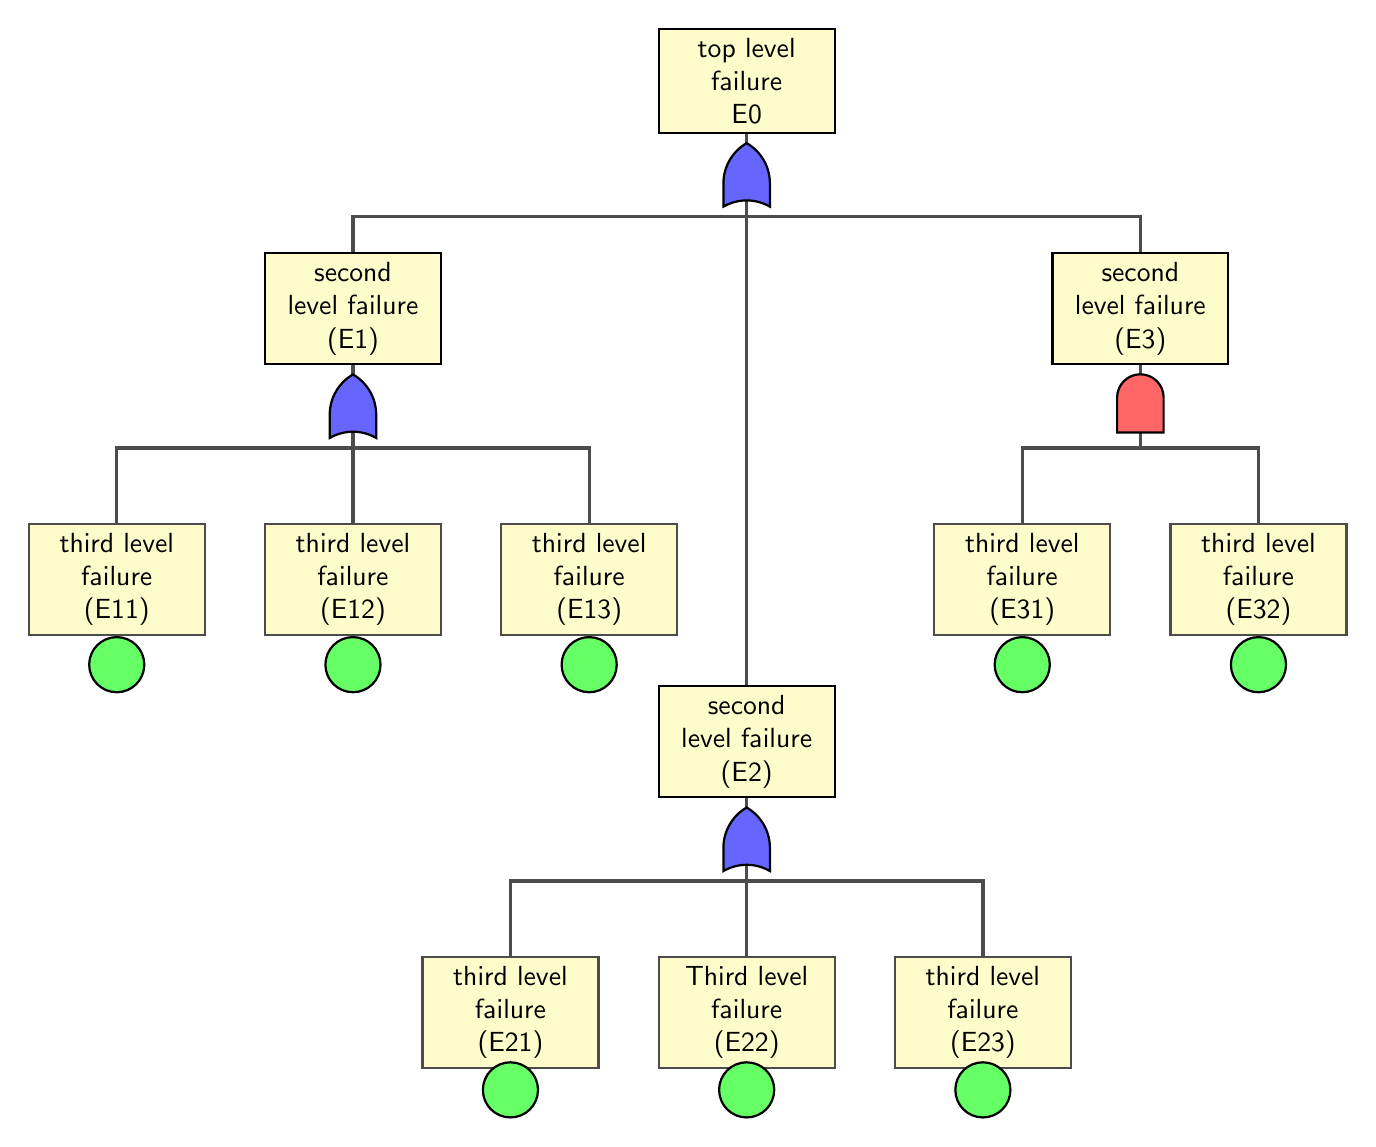
\begin{tikzpicture}
 [
% Gates and symbols style
    and/.style={and gate US,thick,draw,fill=red!60,rotate=90,
        anchor=east,xshift=-1mm},
    or/.style={or gate US,thick,draw,fill=blue!60,rotate=90,
        anchor=east,xshift=-1mm},
    be/.style={circle,thick,draw,fill=green!60,anchor=north,
        minimum width=0.7cm},
% Label style
    label distance=3mm,  every label/.style={blue},
% Event style
    event/.style={rectangle,thick,draw,fill=yellow!20,text width=2cm, text centered,font=\sffamily,anchor=north},
% Children and edges style
    edge from parent/.style={very thick,draw=black!70},
    edge from parent path={(\tikzparentnode.south) -- ++(0,-1.05cm)-| (\tikzchildnode.north)},
    level 1/.style={sibling distance=5cm,level distance=1.5cm, growth parent anchor=south,nodes=event},
    level 2/.style={sibling distance=3cm, level distance=2cm},
    level 3/.style={sibling distance=3cm},
    level 4/.style={sibling distance=3cm}
    ]
%% Draw events and edges
 \node (g1) [event] {top level failure\\ E0}
            child{node (e1) {second level failure\\(E1)} 
                child {node (e11) {third level failure \\ (E11)}}
                child {node (e12) {third level failure \\ (E12)}}
                child {node (e13) {third level failure\\ (E13)}}
            }
        child[level distance=70mm]  {node (e2) {second level failure \\(E2)}
            child {node (e21) {third level failure \\ (E21)}}
            child {node (e22) {Third level failure\\ (E22)}}
            child {node (e23) {third level failure \\ (E23)}}
        }
        child {node (e3) {second level failure\\ (E3)}
            child {node (e31) {third level failure\\ (E31)}}
            child {node (e32) {third level failure\\ (E32)}}
        };
%  Remove what follows if no gates are required
   \node [or]   at (g1.south)   []  {};
   \node [or]   at (e1.south)   []  {};
   \node [or]   at (e2.south)   []  {};
   \node [be]  at ([yshift=1mm]e21.south)  []  {};
   \node [be]  at ([yshift=1mm]e22.south)  []  {};
   \node [be]  at ([yshift=1mm]e23.south)  []  {};
   \node [and]  at (e3.south)   []  {};
   \node [be]   at (e11.south)  []  {};
   \node [be]   at (e12.south)  []  {};
   \node [be]   at (e13.south)  []  {};
   \node [be]   at (e31.south)  []  {};
   \node [be]   at (e32.south)  []  {};
\end{tikzpicture}

\end{document}